\chapter{Лабораторная работа №4 (1Ag)\\
Автоматический рефлектометр}

\section{Цель работы}

\begin{enumerate}
    \item Ознакомиться с измерительными приборами, такими как анализатор спектра и генератор сигналов, входящими в состав лабораторной установки, и программами удалённого управления ими.
    \item Изучить метод измерения КСВН, описанный в работе.
    \item Составить протоколы, содержащие результаты измерения КСВН.
\end{enumerate}

% \section{Теоретические сведения}

\section{Практическая часть}

В соответствии с методикой выполним измерения и занесём данные в табл.~\ref{tab:power-reflection}.
\begin{table}[H]
    \centering
    \caption{Выходная мощность}%
    \label{tab:power-reflection}
    \resizebox{\textwidth}{!}{%
        \begin{tabular}{@{}ccccc@{}}
            \toprule
            Частота установленная, МГц & Мощность ХХ, дБм & Мощность КЗ, дБм & Мощность -12$\sim$дБ, дБм & Коэффициент отражения \\ \midrule
            \rowcolor[HTML]{EFEFEF}
            500                        & -18.12           & -17.68           & -40.38                    & 3.512                 \\
            900                        & -18.05           & -18.05           & -40.10                    & 3.558                 \\
            \rowcolor[HTML]{EFEFEF}
            1400                       & -18.33           & -18.08           & -39.68                    & 3.369                 \\
            1900                       & -17.86           & -18.76           & -42.76                    & 4.416                 \\
            \rowcolor[HTML]{EFEFEF}
            2400                       & -18.48           & -18.02           & -40.50                    & 3.459                 \\ \bottomrule
        \end{tabular}%
    }
\end{table}

На основе полученных данных построим зависимость коэффициента отражения от частоты генератора (Рис.~\ref{fig:reflection}).
\begin{figure}[H]
    \centering
    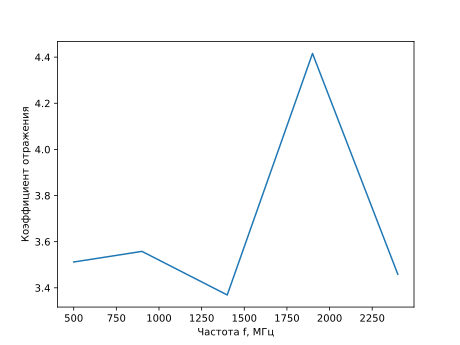
\includegraphics[width=0.8\textwidth]{reflection.pdf}
    \caption{Зависимость коэффициента отражения от частоты}%
    \label{fig:reflection}
\end{figure}


\section{Ответы на вопросы}

\begin{enumerate}
    \item
        Что такое коэффициент отражения?

        \emph{Ответ.}
        Коэффициентом отражения называется отношение отражённой и входной мощностей.
        Коэффициент отражения говорит о том, насколько хорошо согласована нагрузка с генератором.

    \item
        Чему равен коэффициент отражения согласованной нагрузки?

        \emph{Ответ.}
        Коэффициент отражения согласованной нагрузки равен нулю.

    \item
        Как вычислить значение коэффициента стоячей волны по напряжению (КСВН)?

        \emph{Ответ.}
        КСВН может быть определён из выражения
        \[
            \text{КСВН} =
            \frac{E_\text{пад} + E_\text{отр}}{E_\text{пад} - E_\text{отр}} =
            \frac{E_{\max}}{E_{\min}}.
        \]

    \item
        Чему равен коэффициент стоячей волны по напряжению (КСВН) согласованной нагрузки?

        \emph{Ответ.}
        КСВН согласованной нагрузки равен 1.

    \item
        Имеется ли связь между коэффициентом стоячей волны по напряжению (КСВН) и коэффициентом отражения ($\Gamma$)?
        Если имеется, то какая?

        \emph{Ответ.}
        Имеется.
        Между КСВН и коэффициентом отражение существует взамно-однозначное соответствие, определяемое выражением
        \[
            \Gamma =
            \frac{\text{КСВН} - 1}{\text{КСВН} + 1}.
        \]

    \item
        В чём заключается принцип измерений комплексного коэффициента отражения $\dot{\Gamma}$?

        \emph{Ответ.}
        Для измерения $\dot{\Gamma}$ необходимо найти отношение комплексных амплитуд $\dot{E}_\text{пад}$ и $\dot{E}_\text{отр}$.

    \item
        Что такое рефлектометр?

        \emph{Ответ.}
        Рефлектометром называют устройство, необходимое для измерения модуля коэффициента отражения.

    \item
        На чём основан метод измерений модуля коэффициента отражения <<по определению>>?

        \emph{Ответ.}
        Для измерения $\dot{\Gamma}$ <<по определению>> необходимо найти отношение модулей $\dot{E}_\text{пад}$ и $\dot{E}_\text{отр}$, а также разность их фаз, после чего перемножить полученные значения.
\end{enumerate}
